%-----------------------------------------------------------------------
\chapter{Results}
In this chapter we present our final facial animation result, highlight its strengths and weaknesses, and compare the results we have produced throughout the course of this project.

Overall, our final animation resembles the facial performance of the actor quite well. A selection of image frames from the finished render are shown in Figure~\ref{fig:results1}, along side the corresponding poses of the actor. The animation plays at $60$ frames-per-second and it is fluid and expressive - see the final video in the supplementary material. It is perhaps surprising how well the resulting facial animation respects the intrinsic differences between the actor's face shape and Emily's face shape, i.e. the animated expressions are not exact replicas of the actor's expressions, but instead they are Emily versions of the actor's expressions. As we can see in the images in Figure~\ref{fig:results1} the blendshape model is able to capture the extreme facial movements of the actor, including opening the mouth wide, funneling of the lips and scrunching of the face. It is clear that by using the 3D positions of markers on the face rather than simply their 2D positions from a single-view sequence, we able to capture the full 3D motion of the actor's face, for example note the slight forward jutting movement of the jaw in the bottom image. This gives the final facial animation much more nuance and character, and ultimately contributes to a much more believable animation.

Our early animations were generated by solely transferring the computed blendshape weights onto the Emily rig in \Maya. However the resulting animations appeared slightly life-less and dull as the animations did not include subtle movements such as blinking of the eyes, the eye motion, and any movement of the head - giving the animation a slightly robotic appearance. The final result was enhanced by manually activating the blendshapes that control blinks and winks throughout the sequence, an example of which is shown in Figure~\ref{fig:results2a}. We simply analysed the reference video and noted the frames in which the eyelid start to close and open again. Since we tracked points on the face just around the eyes, when the actor blinks the muscles around the eyes move in and this is captured by the blendshape animation quite well. When combined with the manually added eyelid movement this gives a very impressive and natural looking motion. Moreover, when we reintroduced the rigid-head motion that was removed before solving for blendshape weights (see Section~\ref{sec:stabilising_head_movement}), the animation immediately became much more dynamic, see Figure~\ref{fig:results3}.

\begin{figure}
        \centering
        \begin{subfigure}[t]{0.7\textwidth}
                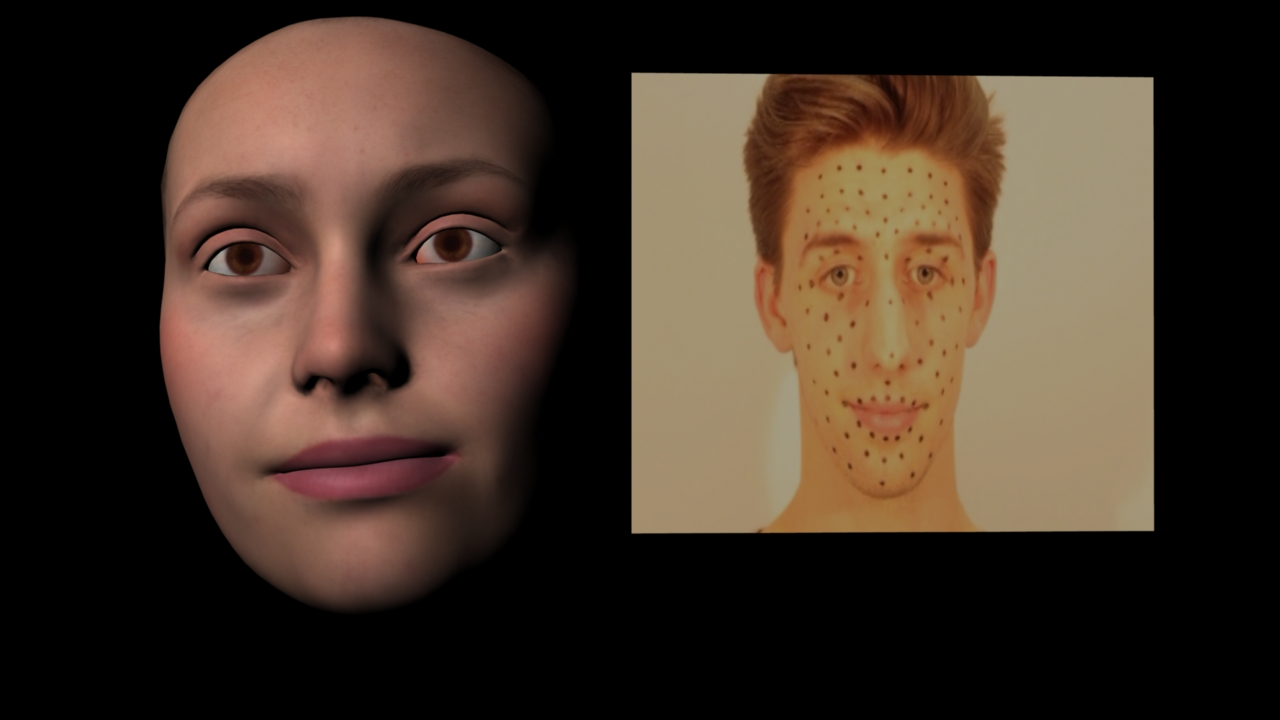
\includegraphics[width=\textwidth]{img/results/Emily_Maya_clean_video_300}
        \end{subfigure}
        \begin{subfigure}[t]{0.7\textwidth}
                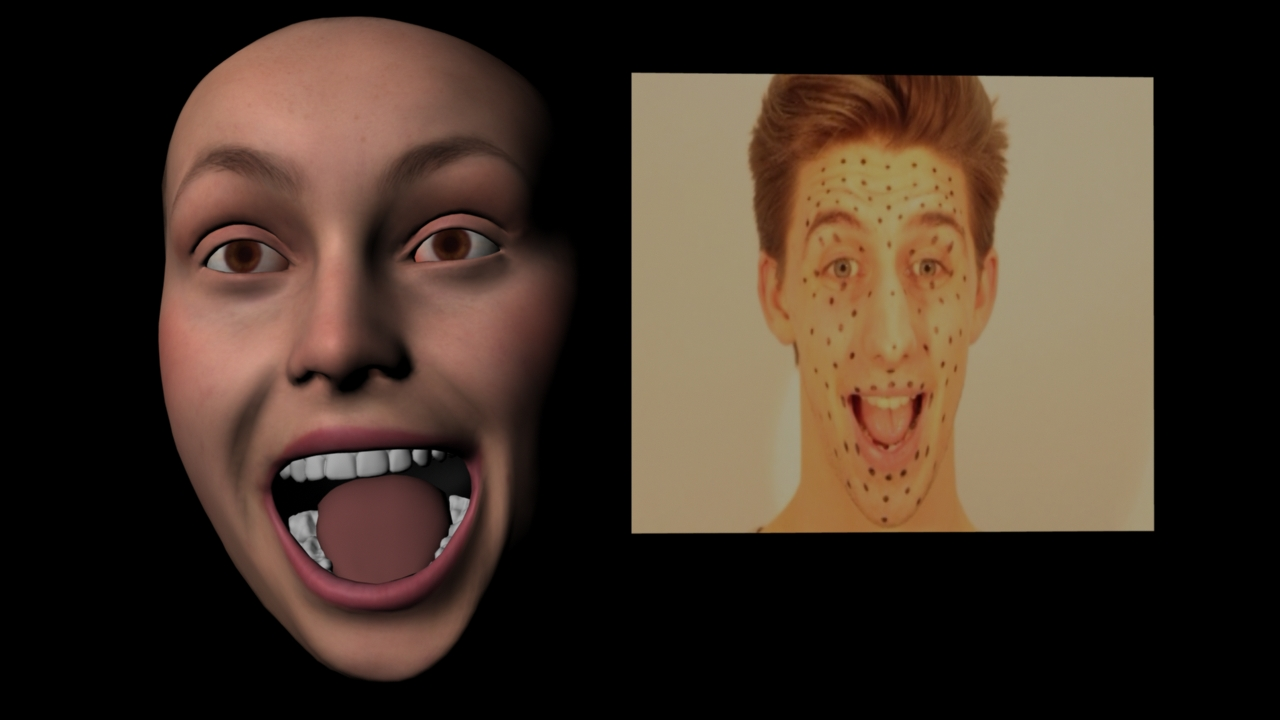
\includegraphics[width=\textwidth]{img/results/Emily_Maya_clean_video_1187}
        \end{subfigure}\\
        \begin{subfigure}[t]{0.7\textwidth}
                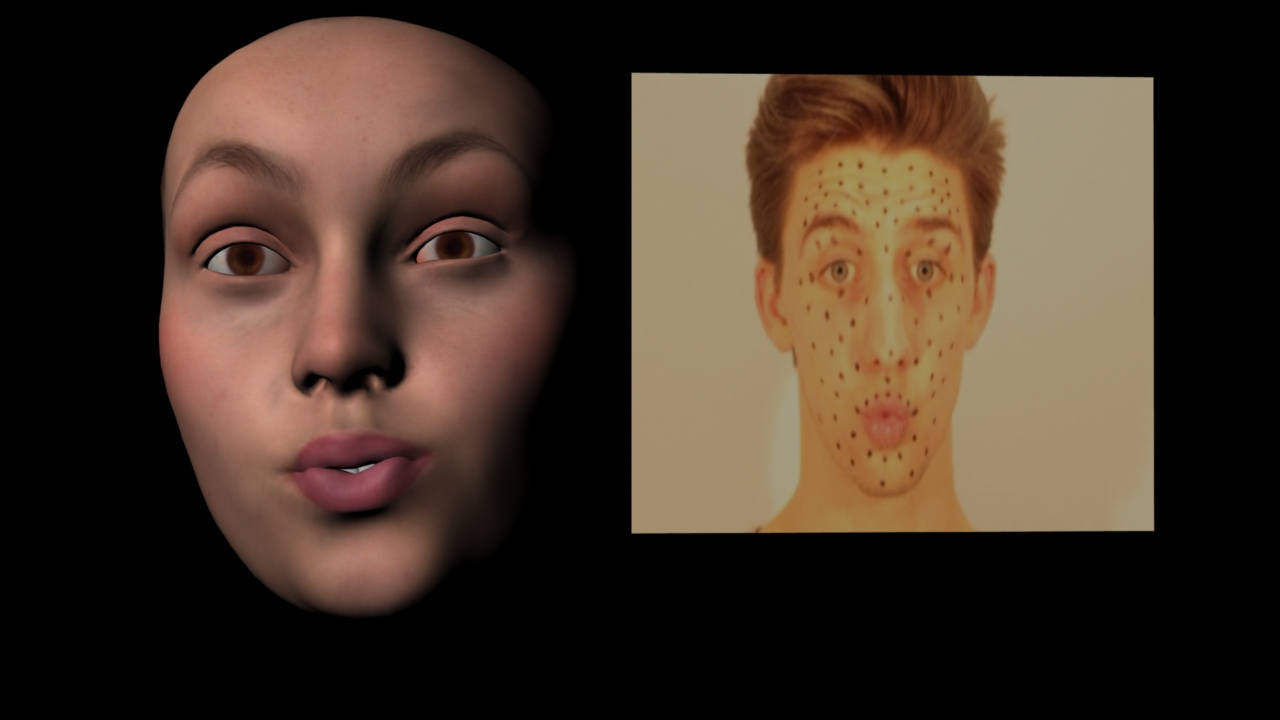
\includegraphics[width=\textwidth]{img/results/Emily_Maya_clean_video_1544}
        \end{subfigure}
        \begin{subfigure}[t]{0.7\textwidth}
                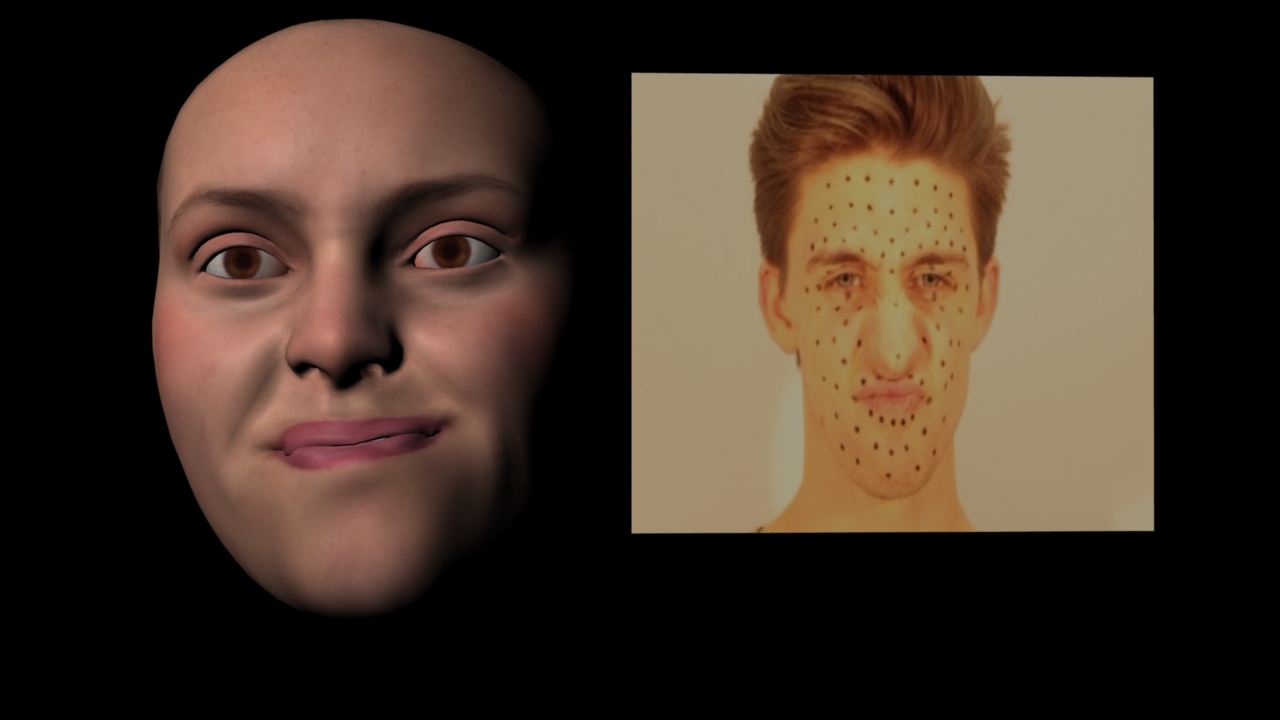
\includegraphics[width=\textwidth]{img/results/Emily_Maya_clean_video_2135}
        \end{subfigure}
        \caption{The final animation well resembles the captured sequence.}
        \label{fig:results1}
\end{figure}
\begin{figure}
        \centering
        \begin{subfigure}[t]{0.5\textwidth}
                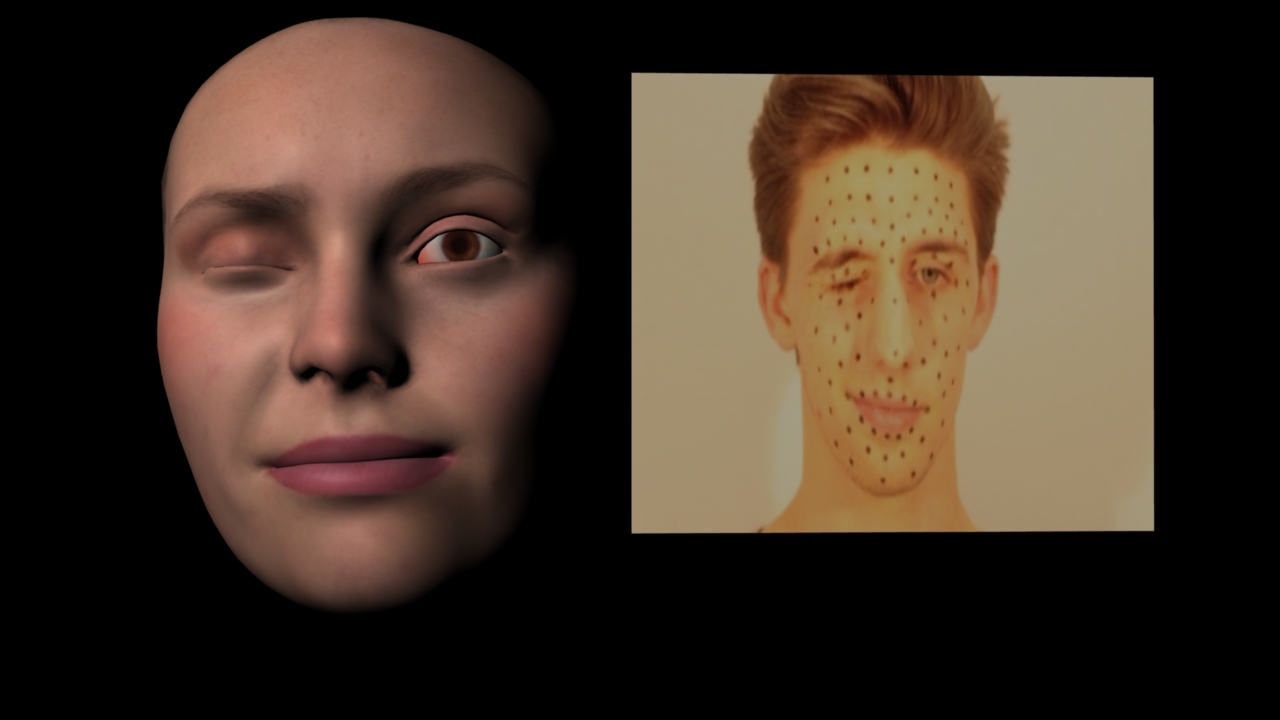
\includegraphics[width=\textwidth]{img/results/Emily_Maya_clean_video_775}
                \caption{Manually added blinks.}\label{fig:results2a}
        \end{subfigure}
        \begin{subfigure}[t]{0.5\textwidth}
                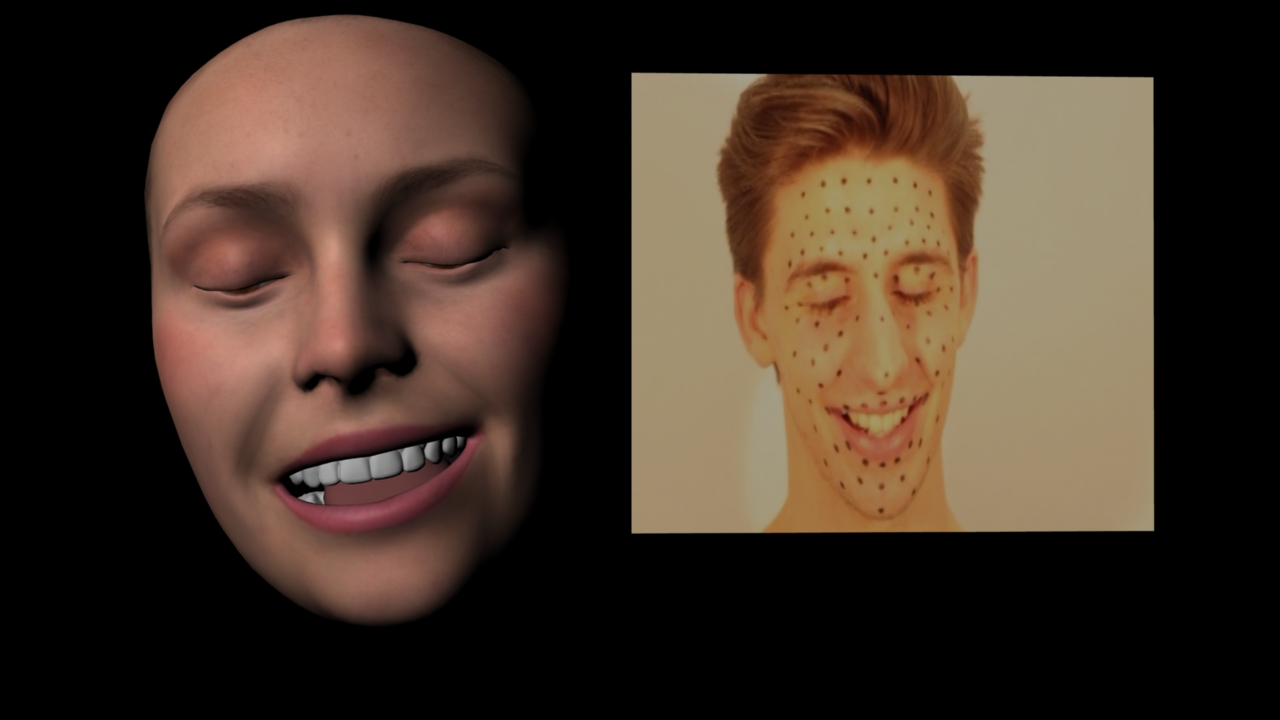
\includegraphics[width=\textwidth]{img/results/Emily_Maya_clean_video_2941}
                \caption{Reintroduced the head rotation.}
        \end{subfigure}
        \caption{Improvements to the blendshape model.}\label{fig:results2b}
        \label{fig:results2}
\end{figure}

However, the final animation does have a number of flaws. First, since only a sparse set of points is used to find the blendshape weights, some motion remains poorly captured. For instance, the expression in Figure~\ref{fig:results3a} presents such a situation. Here the sparse points alone are unable to define the downward positioning of the mouth; the sparse markers around the mouth form a ellipse which is then replicated by Emily without taking into consideration the fact that the actor's mouth is shut. This problem could be solved by actually tracking the inner edge of the lips so that we know when the mouth is actually open or closed.

Another issue is visible in Figure~\ref{fig:results3b}, where the specific combination of blendshape weights here has caused the spherical structure that represents the inside of the mouth to penetrate through the side of Emily's cheek. Unfortunately, we have no control over the motion of this inner structure, and it cannot be hidden since in the \Maya rig it is connected to the mesh of the face. Our approach to this problem involves limiting the upper bound on the weights to ensure that the combination of blendshapes that cause this problem does not occur; by trial and error we were able to eliminate most of the problematic mixtures of shapes.

The final animation is of a much higher quality than our previous results and the way Emily's face moves is much closer to that of the actor's. This is partly due to the method we use to solve for the blendshape weights. In earlier approaches we would transform the sparse performance of the actor using thin plate splines to get an estimate of Emily's sparse performance, and then solve for expressions made by the actor using the Emily blendshapes. But by using the given Emily blendshapes we found that computing a similar set of blendshapes for the actor and solving for the actor's expressions using the generated sparse blendshapes gave a much more plausible set of facial expressions than solving for the actor's expressions in the Emily domain. Usually in industry when doing performance-driven facial animation, we would have a blendshape model of the actor's face and we would solve for the actor's expressions using that model. The problem then becomes just a retargeting problem to transfer the computed blendshape expressions from one model to another. 

\begin{figure}
        \centering
        \begin{subfigure}[t]{0.5\textwidth}
                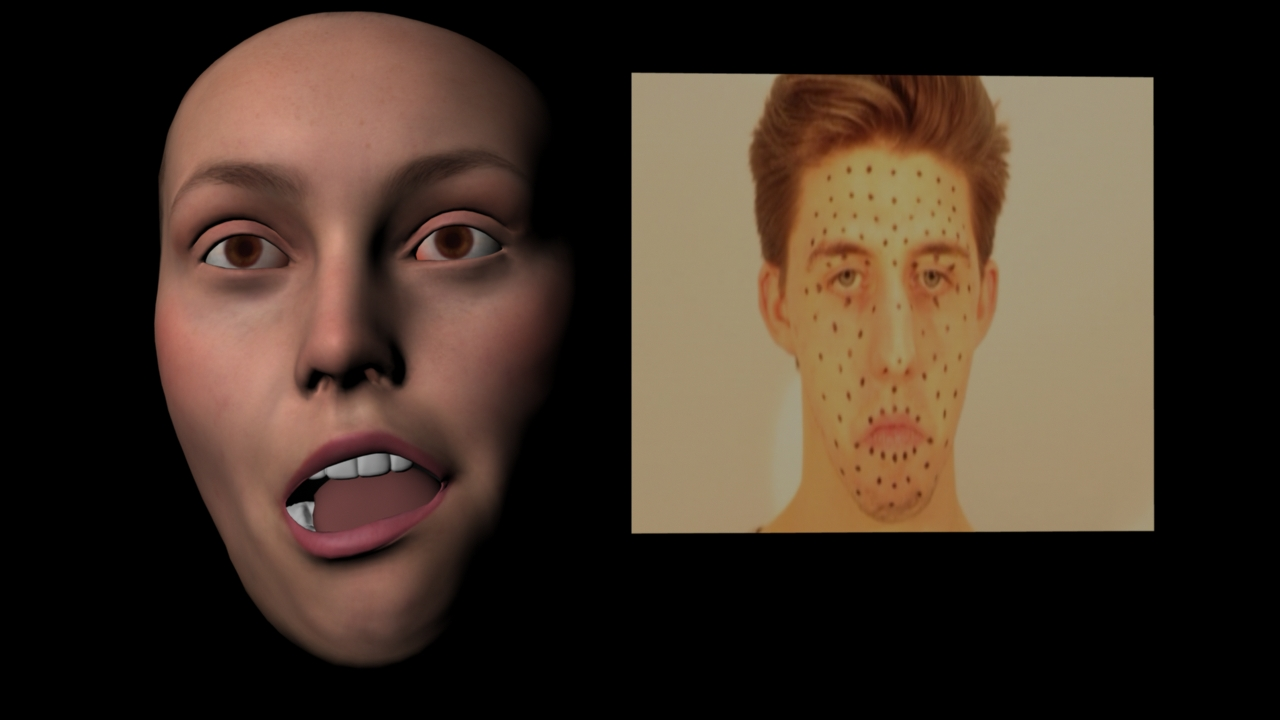
\includegraphics[width=\textwidth]{img/results/Emily_Maya_clean_video_2578}
        \caption{Sparse data does not describe the motion fully.}\label{fig:results3a}
        \end{subfigure}
        \begin{subfigure}[t]{0.5\textwidth}
                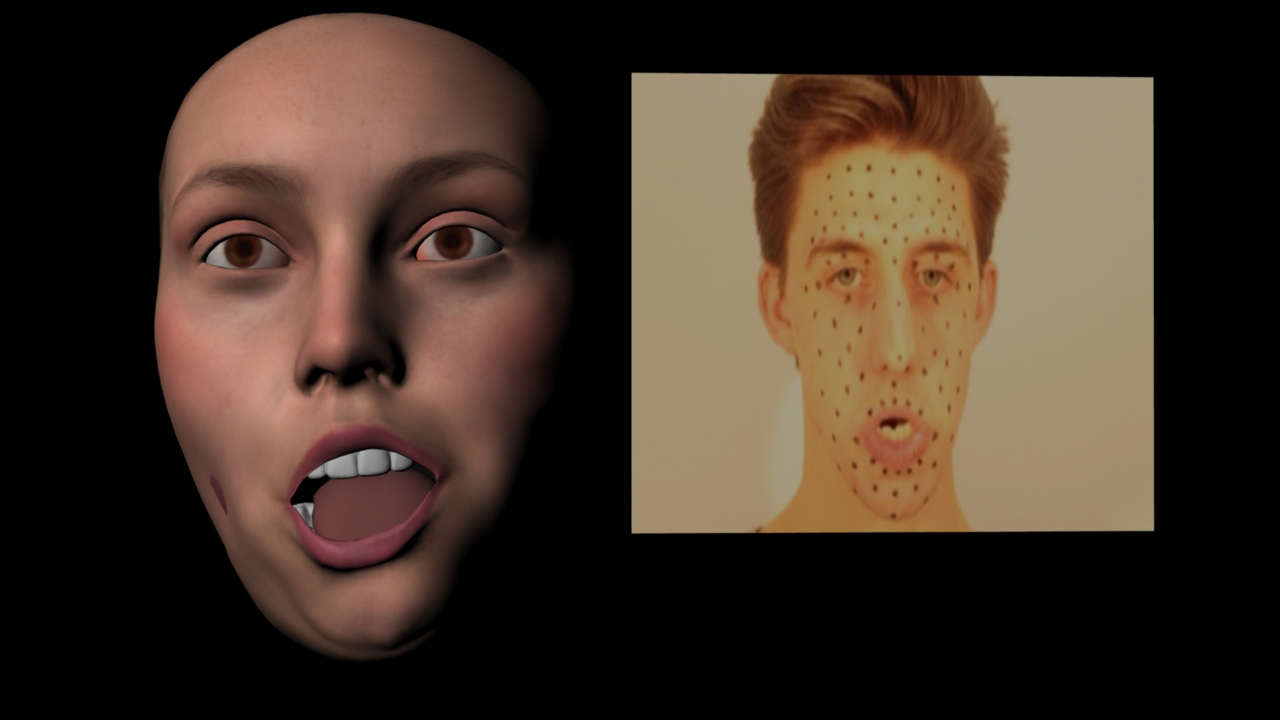
\includegraphics[width=\textwidth]{img/results/Emily_Maya_clean_video_2631}
		\caption{The mesh inside the mouth is allowed to penetrate itself.}\label{fig:results3b}        
        \end{subfigure}
        \caption{Shortcomings of the current model.}
        \label{fig:results3}
\end{figure}